\section{Лабараторная работа №3}

Дадзеная лабараторная работа выконваецца на базе практычнага занятку №3.

\subsection{Структура праекта}

На малюнку \ref{img: lab3} прадстаўлена файлавая структура праекта.

\begin{figure}[h!]
\centering
\begin{subfigure}{0.5\textwidth}
    \centering
    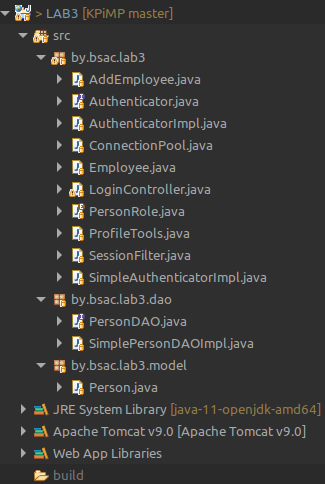
\includegraphics[width=\textwidth]{lab3_structure_1}
\end{subfigure}%
\begin{subfigure}{0.5\textwidth}
    \centering
    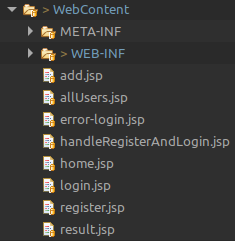
\includegraphics[width=0.7\textwidth]{lab3_structure_2}
\end{subfigure}
\caption{Файлавая структура практычнага занятку}
\label{img: lab3} 
\end{figure}

\subsection{Заданне}

Дабавіць старонку рэгістрацыі, на якой можна зарэгістраваць новага
карыстальніка з усімі патрэбнымі параметрамі.

\subsubsection{Старонка register.jsp}

У лістынгу \ref{lst: lab3_register.jsp} прадстаўлена старонка 
\textit{register.jsp}.

\lstinputlisting[caption={Старонка register.jsp},%
                 label={lst: lab3_register.jsp},%
                 language=HTML5,%
                 style=htmlcssjs]{LAB3/JSP/register.jsp}


\subsubsection{Старонка handleRegisterAndLogin.jsp}

У лістынгу \ref{lst: lab3_handleRegisterAndLogin.jsp} прадстаўлена старонка 
\textit{handleRegisterAndLogin.jsp}.

\lstinputlisting[caption={Старонка handleRegisterAndLogin.jsp},%
                 label={lst: lab3_handleRegisterAndLogin.jsp},%
                 language=HTML5,%
                 style=htmlcssjs]{LAB3/JSP/handleRegisterAndLogin.jsp}
